% Template for ICASSP-2010 paper; to be used with:
%          spconf.sty  - ICASSP/ICIP LaTeX style file, and
%          IEEEbib.bst - IEEE bibliography style file.
% --------------------------------------------------------------------------
\documentclass{article}
\usepackage{spconf,amsmath,graphicx}
\usepackage{url}

% Example definitions.
% --------------------
\def\x{{\mathbf x}}
\def\L{{\cal L}}

% Title.
% ------
\title{IMPUTATION OF BEAT-ALIGNED FEATURES AND MUSIC PATTERN LEARNING}
%
% Single address.
% ---------------
%\name{Thierry Bertin-Mahieux\thanks{Thanks to NSERC and some other stuff.}}
%\address{EE dept., Columbia University}
%
% For example:
% ------------
%\address{School\\
%	Department\\
%	Address}
%
% Two addresses (uncomment and modify for two-address case).
% ----------------------------------------------------------
\twoauthors
  {Thierry Bertin-Mahieux\sthanks{TBM is supported in part by a NSERC PG scholarship.}, Ron J. Weiss\sthanks{Thanks something}}
	{Columbia University / New York University\\
          LabROSA / MARL\\
	New York, USA}
  {Graham Grindlay and Daniel P.W. Ellis}
	{Columbia University\\
          LabROSA\\
	New York, USA}

\begin{document}
%\ninept
%
\maketitle
%
\begin{abstract}
Imputation is cool. It is a well-defined problem, as opposed to segmentation.
Gives a reasonable benchmark to compare algorithms that claim learning meaningful
patterns on music. Hard to beat benchmarks comparison, for instance linear
prediction. We compare some methods and discuss contradicting error measures. 
We'll track you down if you don't accept this paper.
\end{abstract}
%
\begin{keywords}
Missing data, chroma features, beat imputation, codebook learning
\end{keywords}
%
\section{Introduction}
\label{sec:intro}
Many signals show similarities and repetitions over time. Learning these repetitions
in an unsupervised way remains a challenge. Finding robust patterns should prove useful in
many tasks like song similarity (songs with similar patterns), song segmentation
(song segments with different patterns) or cover song recognition (songs with exactly
the same patterns).
Therefore, we are looking for patterns that not only explain the signal (in an encoding
framework), but also contain musical characteristics. 

We devise a task that let us measure
the quality of such patterns in an attempt at unifying this research field.
Imputation is a well-studied problem for audio to show that some model can generalize.
However, it has not been pushed as far as it could, and fully masking consecutive beats
of music have not been considered. A real-life analogous problem would be a music stream
signal that is lost for a few seconds. The goal here would be to infer a reasonable
stream to replace the original one. Thus we do not only want a signal close to the original
in a reconstruction sense, but also a signal that has similar ``musical properties'' to
the user ear.

\begin{figure}[t]
\begin{center}
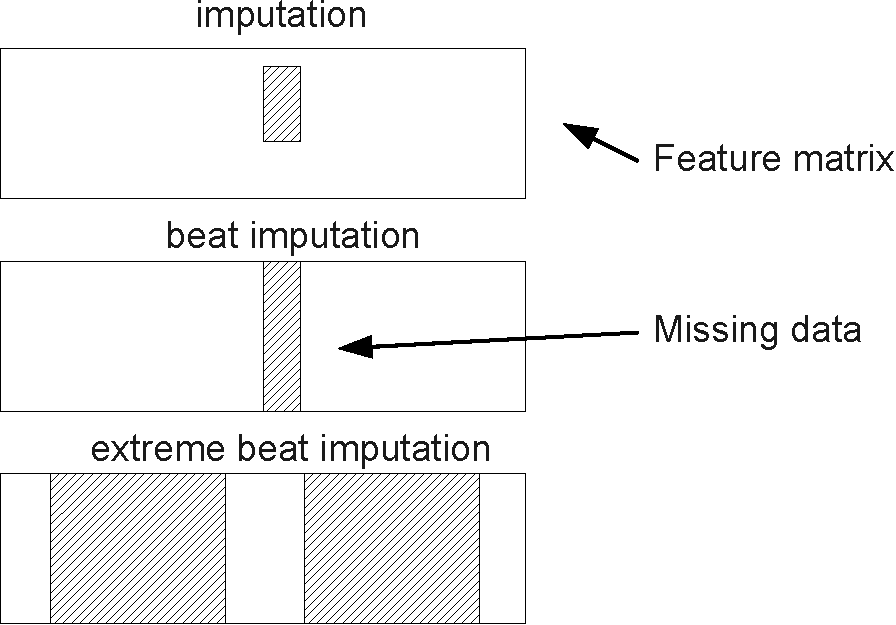
\includegraphics[width=.7\columnwidth]{type_imputation}
\end{center}
\caption{Imputation types.
\label{fig:types}}
\end{figure}

Figure \ref{fig:types} summarizes the difference between different sorts of imputation.
Usually \cite{Smaragdis2009}, a few frequency bins are hidden and can be recovered from
their neighborhood, both in time and frequency. Masking one full beat is a natural extension,
and the solution is easy as music notes are often sustained over many beats. Two or three
missing beats remain solvable as music bare many repetitions. One can usually find a similar
section from an unmasked part of the song (think about a repeated chorus for instance).
The real challenge arises from masking many consecutive beats.

Figure \ref{fig:basic} shows an example of the imputation of $15$ beats on chroma features
(see Section ???). The solution in that figure, although intuitively wrong, is very
accurate according to euclidean distance. As we mentioned above, reconstruction error and
music properties do not agree. Understanding this conflict is essential to the task
definition.

\begin{figure}[t]
\begin{center}
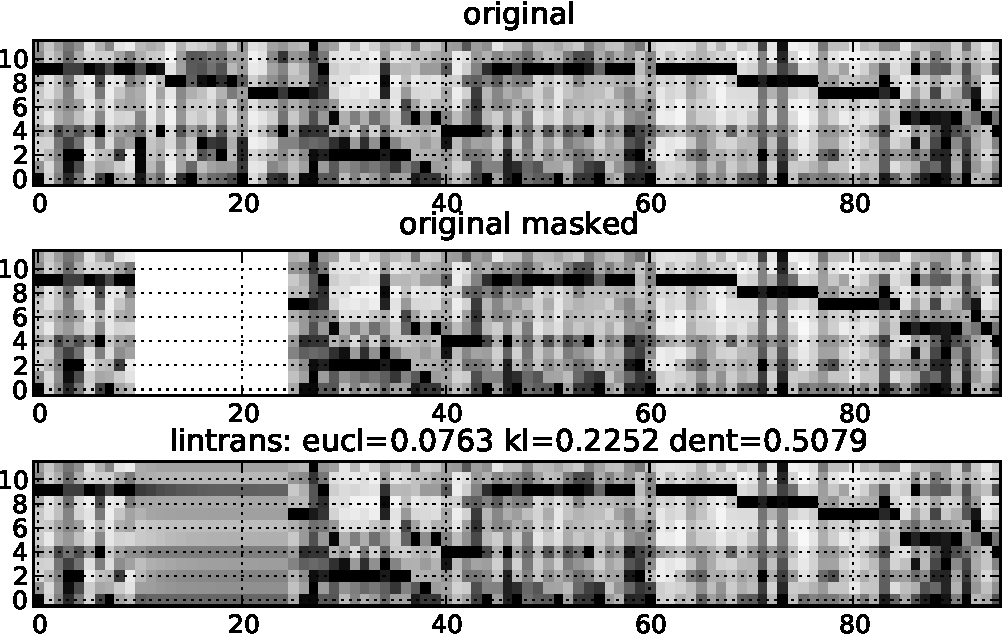
\includegraphics[width=.95\columnwidth]{basic}
\end{center}
\caption{$15$ beats imputation example, rows are 1) original 2) original masked
3) reconstruction using a linear transform of one previous beat.
\label{fig:basic}}
\end{figure}


\subsection{RELATED WORK} 
\label{ssec:relwork}

Prev work by me: \cite{Bertin-Mahieux2010a}. Imputation \cite{Smaragdis2009,Hoffman2010}.


\section{TASK DEFINITION}
\label{sec:task}

\subsection{DATA AND FEATURES}
\label{ssec:feats}
We use beat-aligned chroma features \cite{Ellis2007a}. Chroma features
record the intensity associated with each of the 12 semitones
(e.g. piano keys) within one octave, but all octaves
are folded together. One can see them as a very coarse and
noisy music transcription. They have been used for segmentation, 
chord recognition and cover recognition
among others. The specific implementation we use is the one
returned by the Echo Nest API \cite{EchoNest} which uses a constant-
Q spectrogram and where the chroma for each time stamp is
normalized so the max is 1. We use a random subset of $5K$ songs of
the cowbell dataset \cite{Bertin-Mahieux2010a} in our experiments.

\subsection{MEASURES}
\label{ssec:measures}
The choice of measure function is closely related to the properties
we expect to preserve in learned patterns. As we saw in Figure
\ref{fig:basic}, reconstruction error does not tell the whole story.
We present different error measures and look at what imputation they
favor.

Euclidean, entropy, delta, L1, L1/2, your mama.

\begin{figure}[t]
\begin{center}
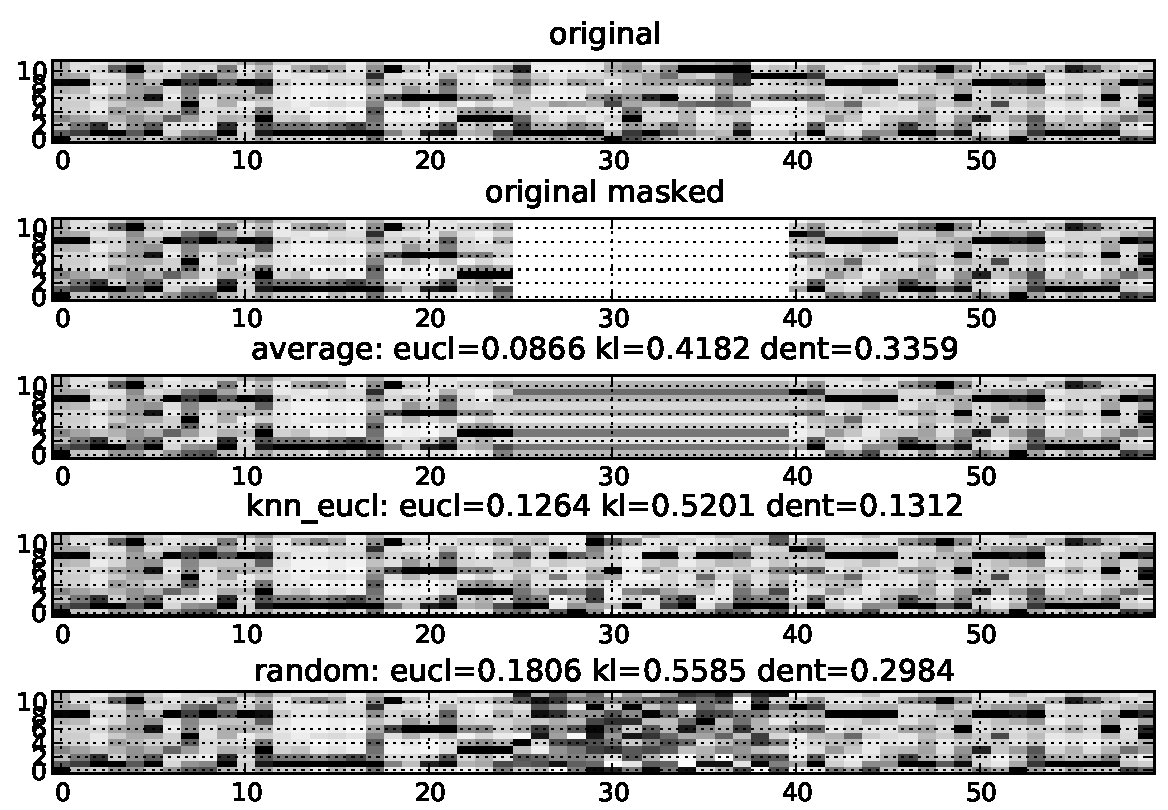
\includegraphics[width=.95\columnwidth]{avg_nn_rand}
\end{center}
\caption{Same beat imputation example as Figure \ref{fig:basic}, 
rows are 1) original 2) original masked
3) reconstruction using the average of nearby beats 4) using
nearest neighbor 5) using random.
\label{fig:avgnnrand}}
\end{figure}


\section{EXPERIMENTS}
\label{sec:exp}
We present results from different algorithms for imputing $1$ to
$15$ beats.

\subsection{ALGORITHMS}
\label{ssec:algo}
Random, average, nearest-neighbor, linear prediction, SIPLCA, HMM,
your mama.

\subsection{RESULTS}
\label{ssec:results}


\begin{figure}[t]
\begin{center}
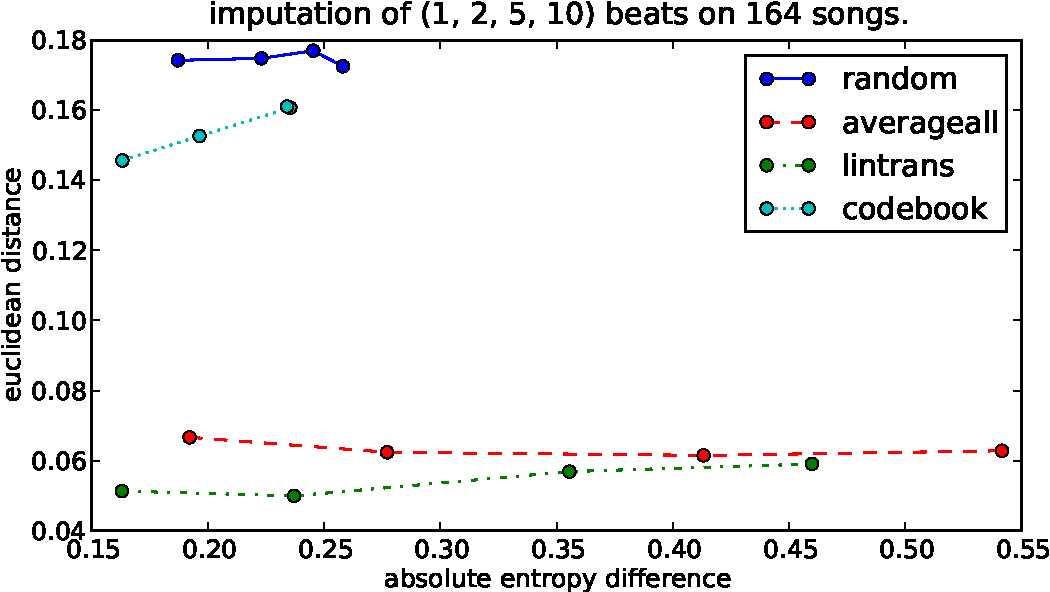
\includegraphics[width=.9\columnwidth]{recon_score_in_2d}
\end{center}
\caption{Reconstruction error for $4$ methods and different
number of masked beats. Errors are ANDE and euclidean
distance. In all cases, the larger the number of masked beats,
the higher the euclidean distance. Lower left is better.
\label{fig:2dscore}}
\end{figure}


\iffalse
\begin{table}[t]
\begin{small}
\begin{center}
\begin{tabular}{l|c|c|c|c|c|}
\# beats  & 1 & 2 & 5 & 10 & 15 \\ \hline \hline
random & $0.166$ & $0.166$ & $0.167$ & $0.167$ & $0.168$  \\
rand. song & $0.115$ & $0.114$ & $0.114$ & $0.115$ & $0.115$  \\
average all & $0.057$ & $0.057$ & $0.057$ & $0.057$ & $0.058$ \\
average & $0.047$ & $0.053$ & $0.062$ & $0.065$ & $0.069$ \\ \hline
knn eucl & $0.048$ & $0.049$ & $0.055$ & $0.064$ &  $0.070$ \\
knn kl & $0.049$ & $0.050$ & $0.056$ & $0.066$ &  $0.071$ \\
lin. trans. & $\mathbf{0.044}$ & $\mathbf{0.047}$ & $\mathbf{0.051}$ & $\mathbf{0.053}$ & $\mathbf{0.055}$ \\
codebook & & & & &  \\
SIPLCA & & & & &  \\ \hline
\end{tabular}
\caption{Results based on euclidean distance on $43K$ songs.
Song has to be at least $70$ beats long. 
For ``average'', window is $2$ beats each side of the masked patch.
For ``knn eucl'' and ``knn kl'', window is $10$ beats each side of the masked patch.
For ``lin. trans.'', window is the $2$ previous beats.}
\label{tab:reseucl}
\end{center}
\end{small}
\end{table}

\begin{table}[t]
\begin{small}
\begin{center}
\begin{tabular}{l|c|c|c|c|c|}
\# beats & 1 & 2 & 5 & 10 & 15 \\ \hline \hline
random & $0.428$ & $0.450$ & $0.461$ & $0.461$ & $0.462$  \\
rand. song & $0.334$ & $0.351$ & $0.371$ & $0.377$ & $0.380$  \\
average all & $0.164$ & $0.175$ & $0.183$ & $0.187$ & $0.189$ \\ 
average & $0.121$ & $0.154$ & $0.194$ & $0.212$ &  $0.223$ \\ \hline
knn eucl & $\mathbf{0.116}$ & $0.136$ & $0.169$ & $0.212$ & $0.233$ \\
knn kl & $\mathbf{0.116}$ & $\mathbf{0.135}$ & $\mathbf{0.167}$ & $0.209$ & $0.229$ \\
lin. trans. & $0.141$ & $0.157$ & $0.170$ & $\mathbf{0.180}$ & $\mathbf{0.184}$ \\
codebook & & & & &  \\
SIPLCA & & & & &  \\ \hline
\end{tabular}
\caption{Results based on symmetric KL divergence on $43K$ songs.
See Table \ref{tab:reseucl} for the exact parameters used.}
\label{tab:reskl}
\end{center}
\end{small}
\end{table}
\fi

\section{CONCLUSION AND FUTURE WORK}
\label{sec:conclusion}


Code available at \footnote{Code available at: \url{http://www.columbia.edu/~tb2332/something}}.



% References should be produced using the bibtex program from suitable
% BiBTeX files (here: strings, refs, manuals). The IEEEbib.bst bibliography
% style file from IEEE produces unsorted bibliography list.
% -------------------------------------------------------------------------
\bibliographystyle{IEEEbib}
\bibliography{tbm_bib}

\end{document}
